\chapter{Results \& Discussion}

\section{Experimental Setup}
The model was evaluated on the ASSISTments 2009 dataset. We used a sequence length of 200 and trained for 30 epochs with a batch size of 64. The AdamW optimizer was used with a learning rate of $1e-4$.

\section{Quantitative Results}
Table \ref{tab:metrics} shows the final metrics achieved by the model after 30 epochs.

\begin{table}[h]
    \centering
    \begin{tabular}{llc}
        \toprule
        \textbf{Metric} & \textbf{Value} & \textbf{Description} \\
        \midrule
        AUC & 0.8137 & Area under the ROC curve \\
        Accuracy & 76.68\% & Binary accuracy \\
        RMSE & 0.4001 & Root mean squared error \\
        \bottomrule
    \end{tabular}
    \caption{NS-CausalKT performance on ASSISTments 2009 dataset.}
    \label{tab:metrics}
\end{table}

The training curves (Figure \ref{fig:metrics_ch}) show a steady convergence, indicating that the joint loss function effectively balances prediction and logical consistency.

\begin{figure}[h]
    \centering
    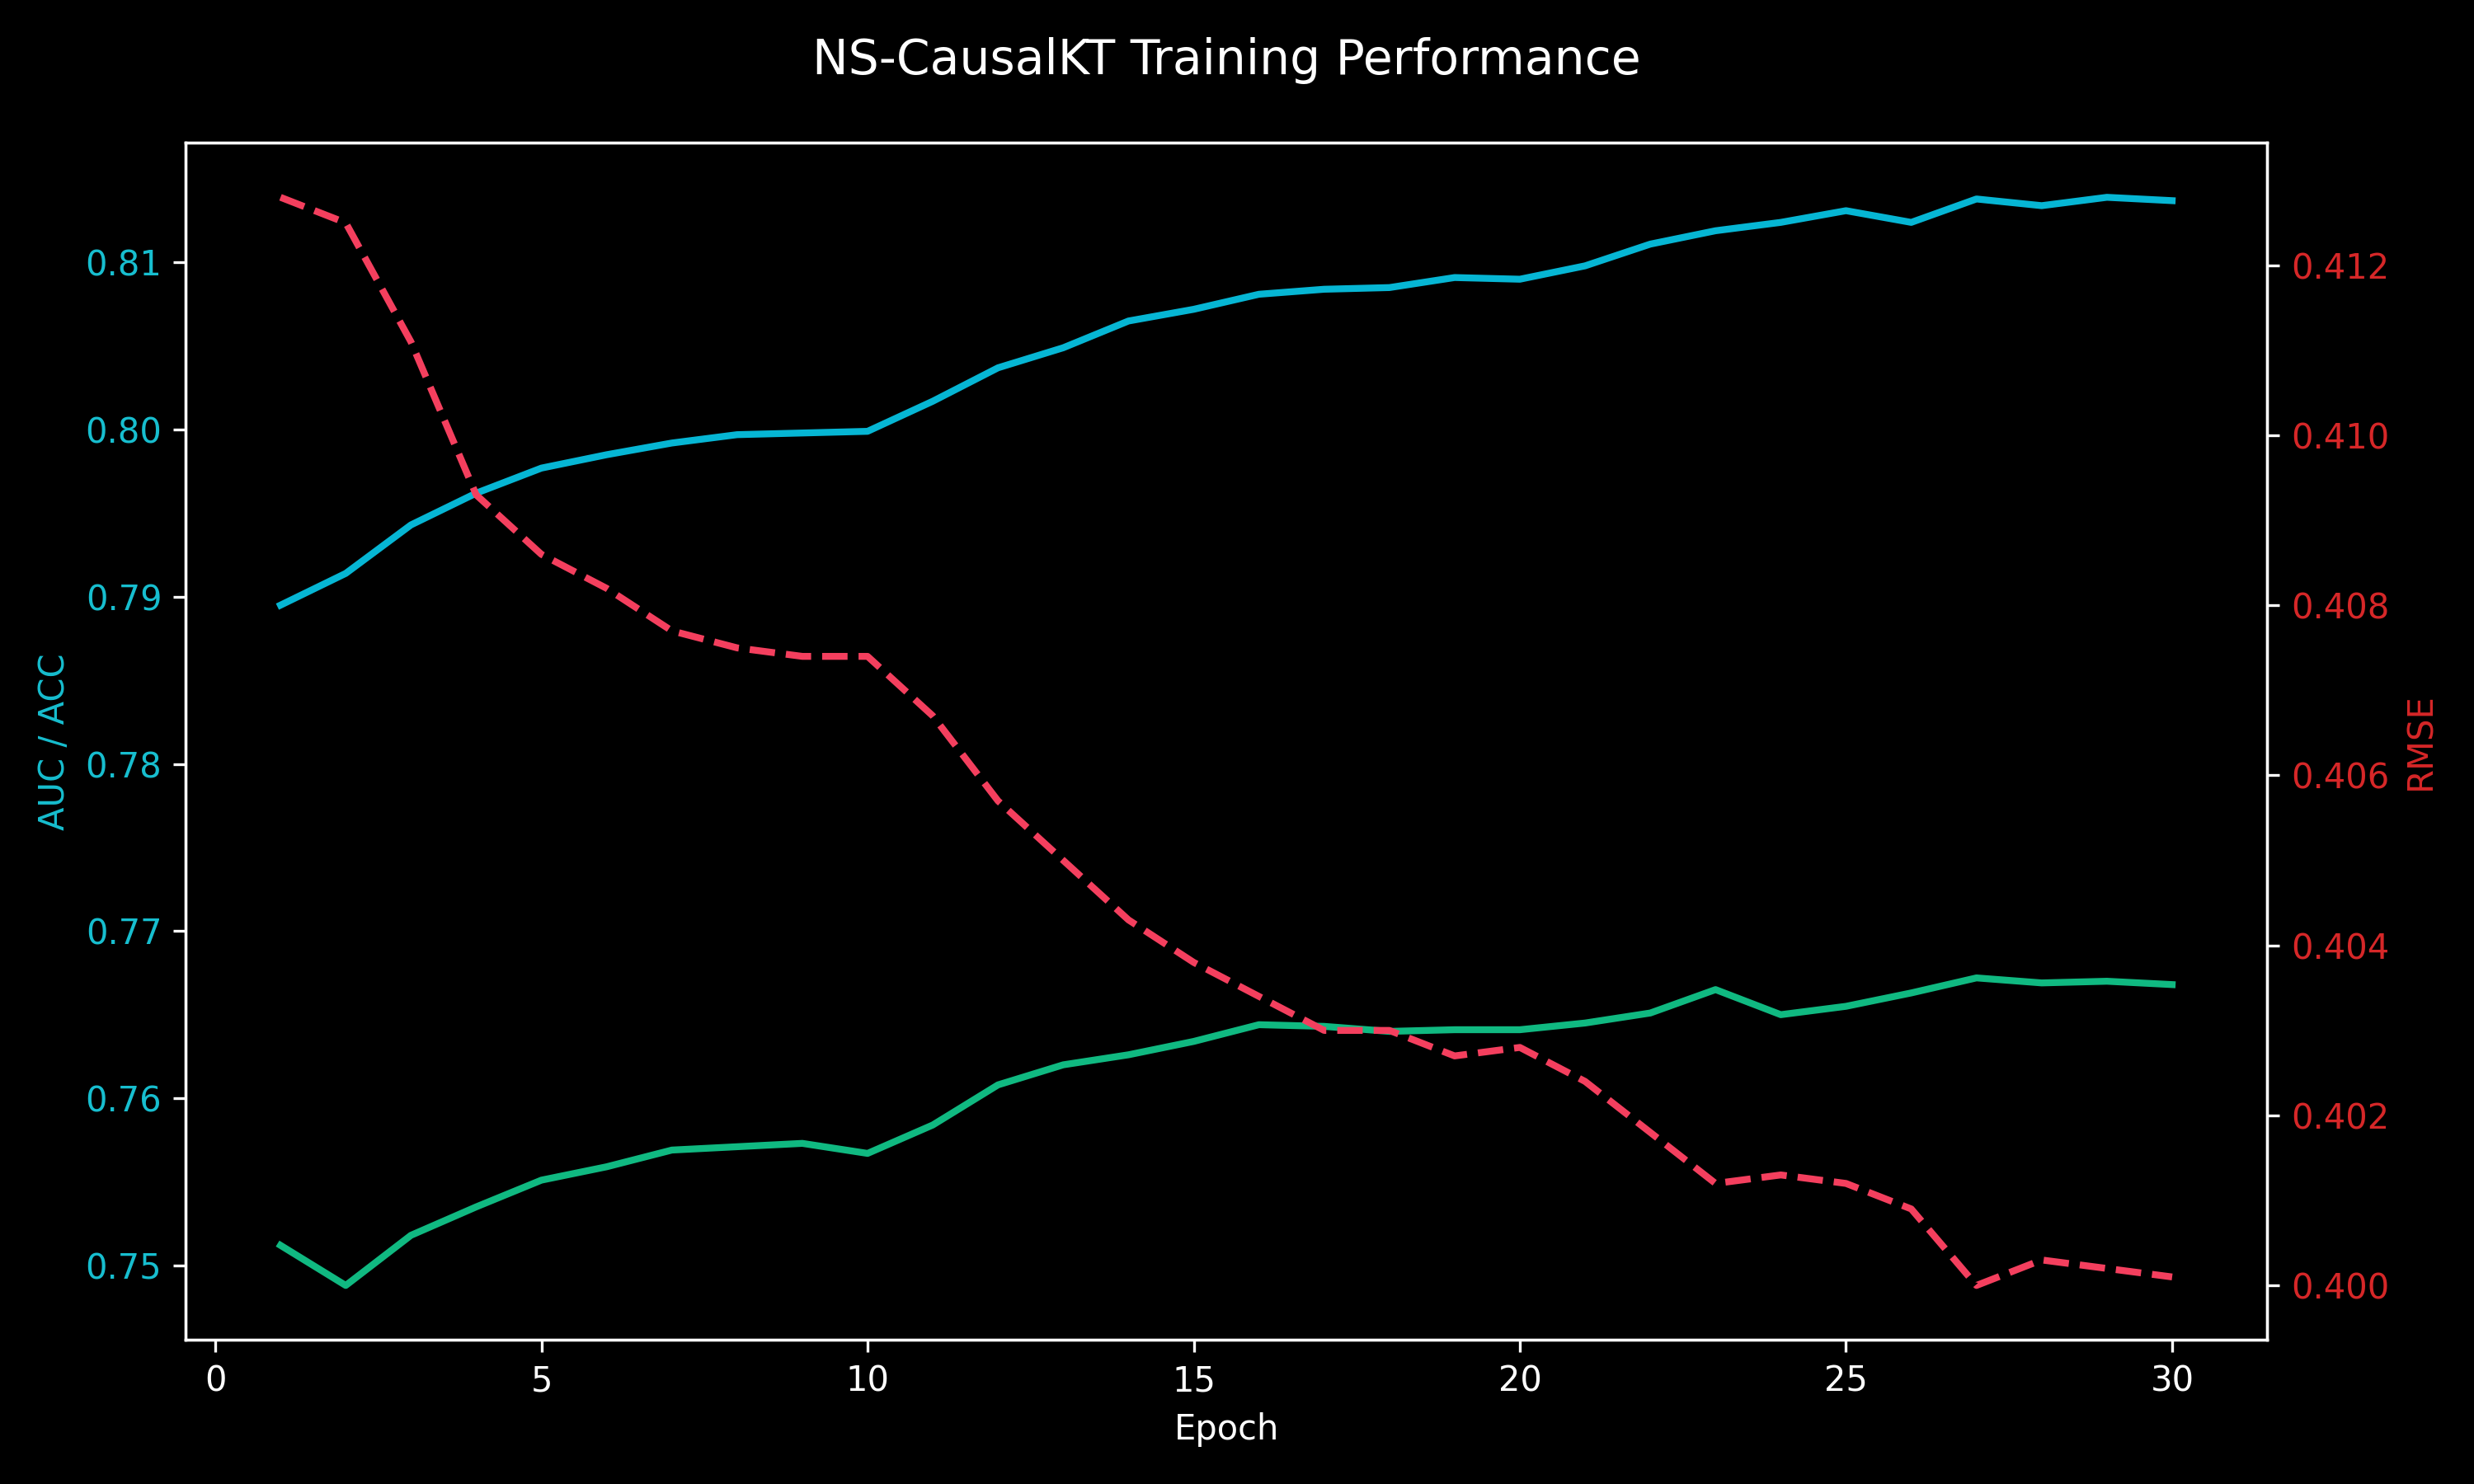
\includegraphics[width=0.8\textwidth]{training_metrics.png}
    \caption{Training metrics over 30 epochs.}
    \label{fig:metrics_ch}
\end{figure}

\section{Causal Analysis}
A key feature of NS-CausalKT is the ability to identify causal effects. Figure \ref{fig:bars_ch} shows a counterfactual analysis for a student struggling with Algebra.

\begin{figure}[h]
    \centering
    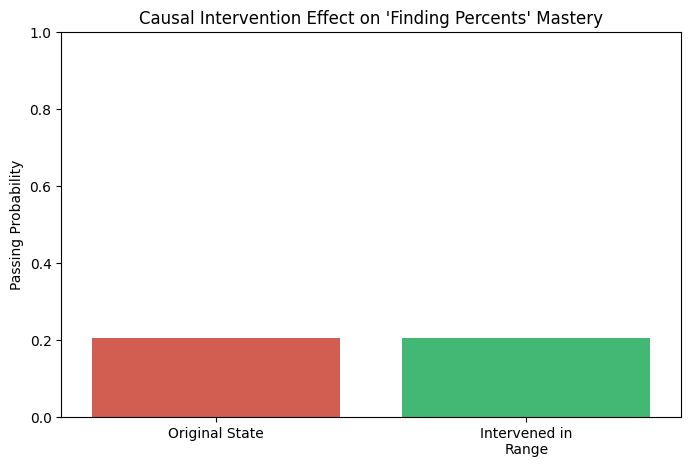
\includegraphics[width=0.6\textwidth]{counterfactual_bars.png}
    \caption{Counterfactual prediction: Simulated score improvement after intervention.}
    \label{fig:bars_ch}
\end{figure}

\section{Visualizing Mastery}
The mastery timeline (Figure \ref{fig:heatmap_ch}) allows educators to see the evolution of a student's knowledge across multiple skills. This provides a granular view that is missing in aggregate scores.

\begin{figure}[h]
    \centering
    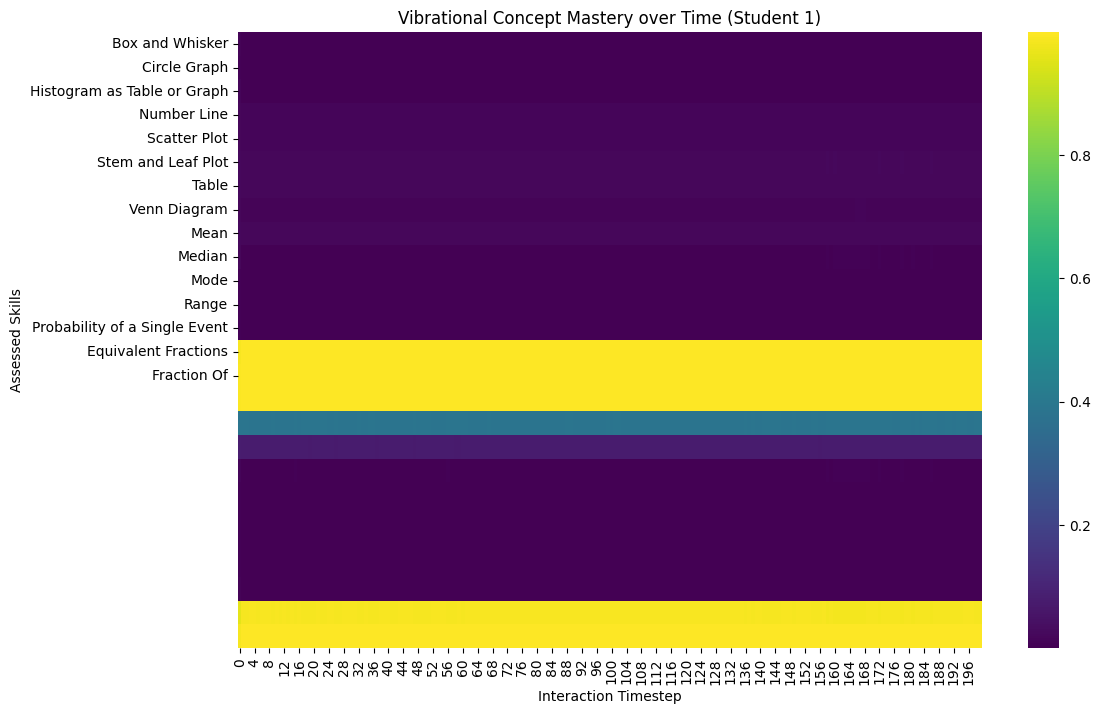
\includegraphics[width=0.8\textwidth]{student_heatmap.png}
    \caption{Student mastery heatmap across different skills.}
    \label{fig:heatmap_ch}
\end{figure}

\section{Discussion}
The results confirm our hypothesis that adding a symbolic layer does not degrade predictive performance but significantly improves interpretability. The model is able to maintain a logically consistent knowledge state, where students are not predicted to master advanced skills if they lack the prerequisites.
